\section{实验一 周期信号的分解与合成}
\subsection{一、实验流程图}
\begin{figure}[H]
\centering
\begin{tikzpicture}[
    node distance=1.6cm,
    auto,
    block/.style={rectangle, draw, text width=8.5em, align=center, minimum height=2.8em}
]
\node [block] (start) {程序初始化};
\node [block,below of=start] (para) {设置信号参数};
\node [block,below of=para] (gen) {生成原始周期信号};
\node [block,below of=gen] (fs) {傅里叶级数合成};
\node [block,below of=fs] (dfs) {离散 DFS/IDFS 分析};
\node [block,below of=dfs] (plot) {绘制波形与频谱};
\node [block,below of=plot] (end) {结束};

\draw[->] (start) -- (para);
\draw[->] (para) -- (gen);
\draw[->] (gen) -- (fs);
\draw[->] (fs) -- (dfs);
\draw[->] (dfs) -- (plot);
\draw[->] (plot) -- (end);
\end{tikzpicture}
\caption{实验一程序流程图}
\end{figure}

\subsection{二、实验结果附图}
\begin{figure}[H]
\centering
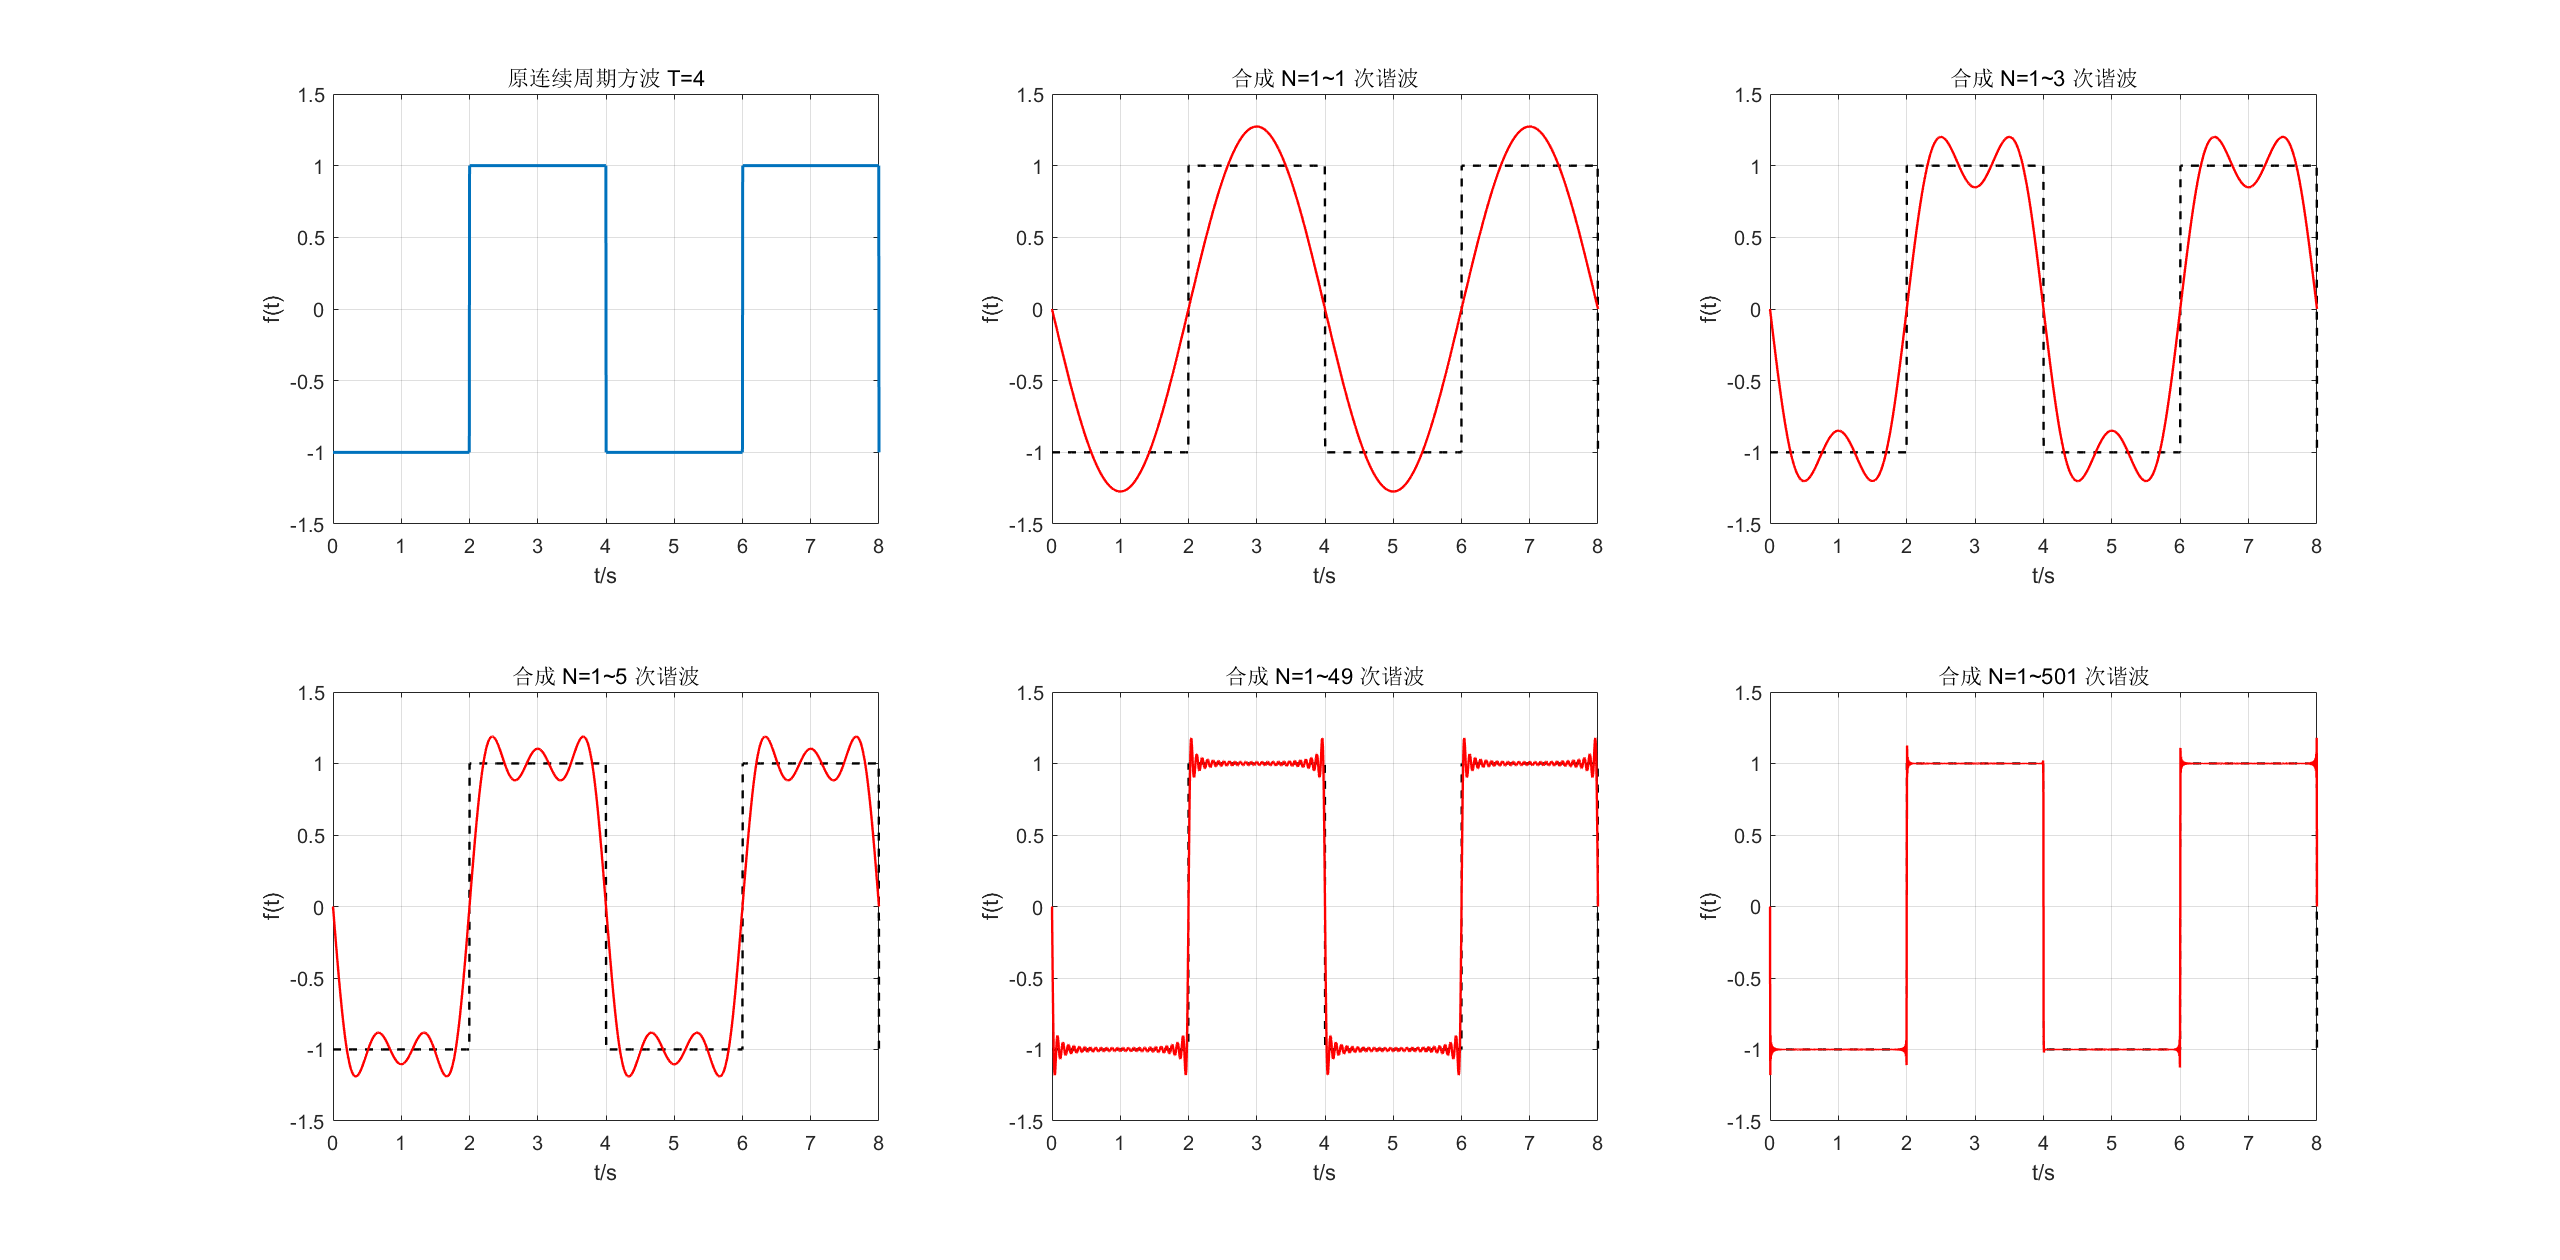
\includegraphics[width=0.8\textwidth]{1.1.png}
\caption{连续周期方波原始时域波形}
\end{figure}

\begin{figure}[H]
\centering
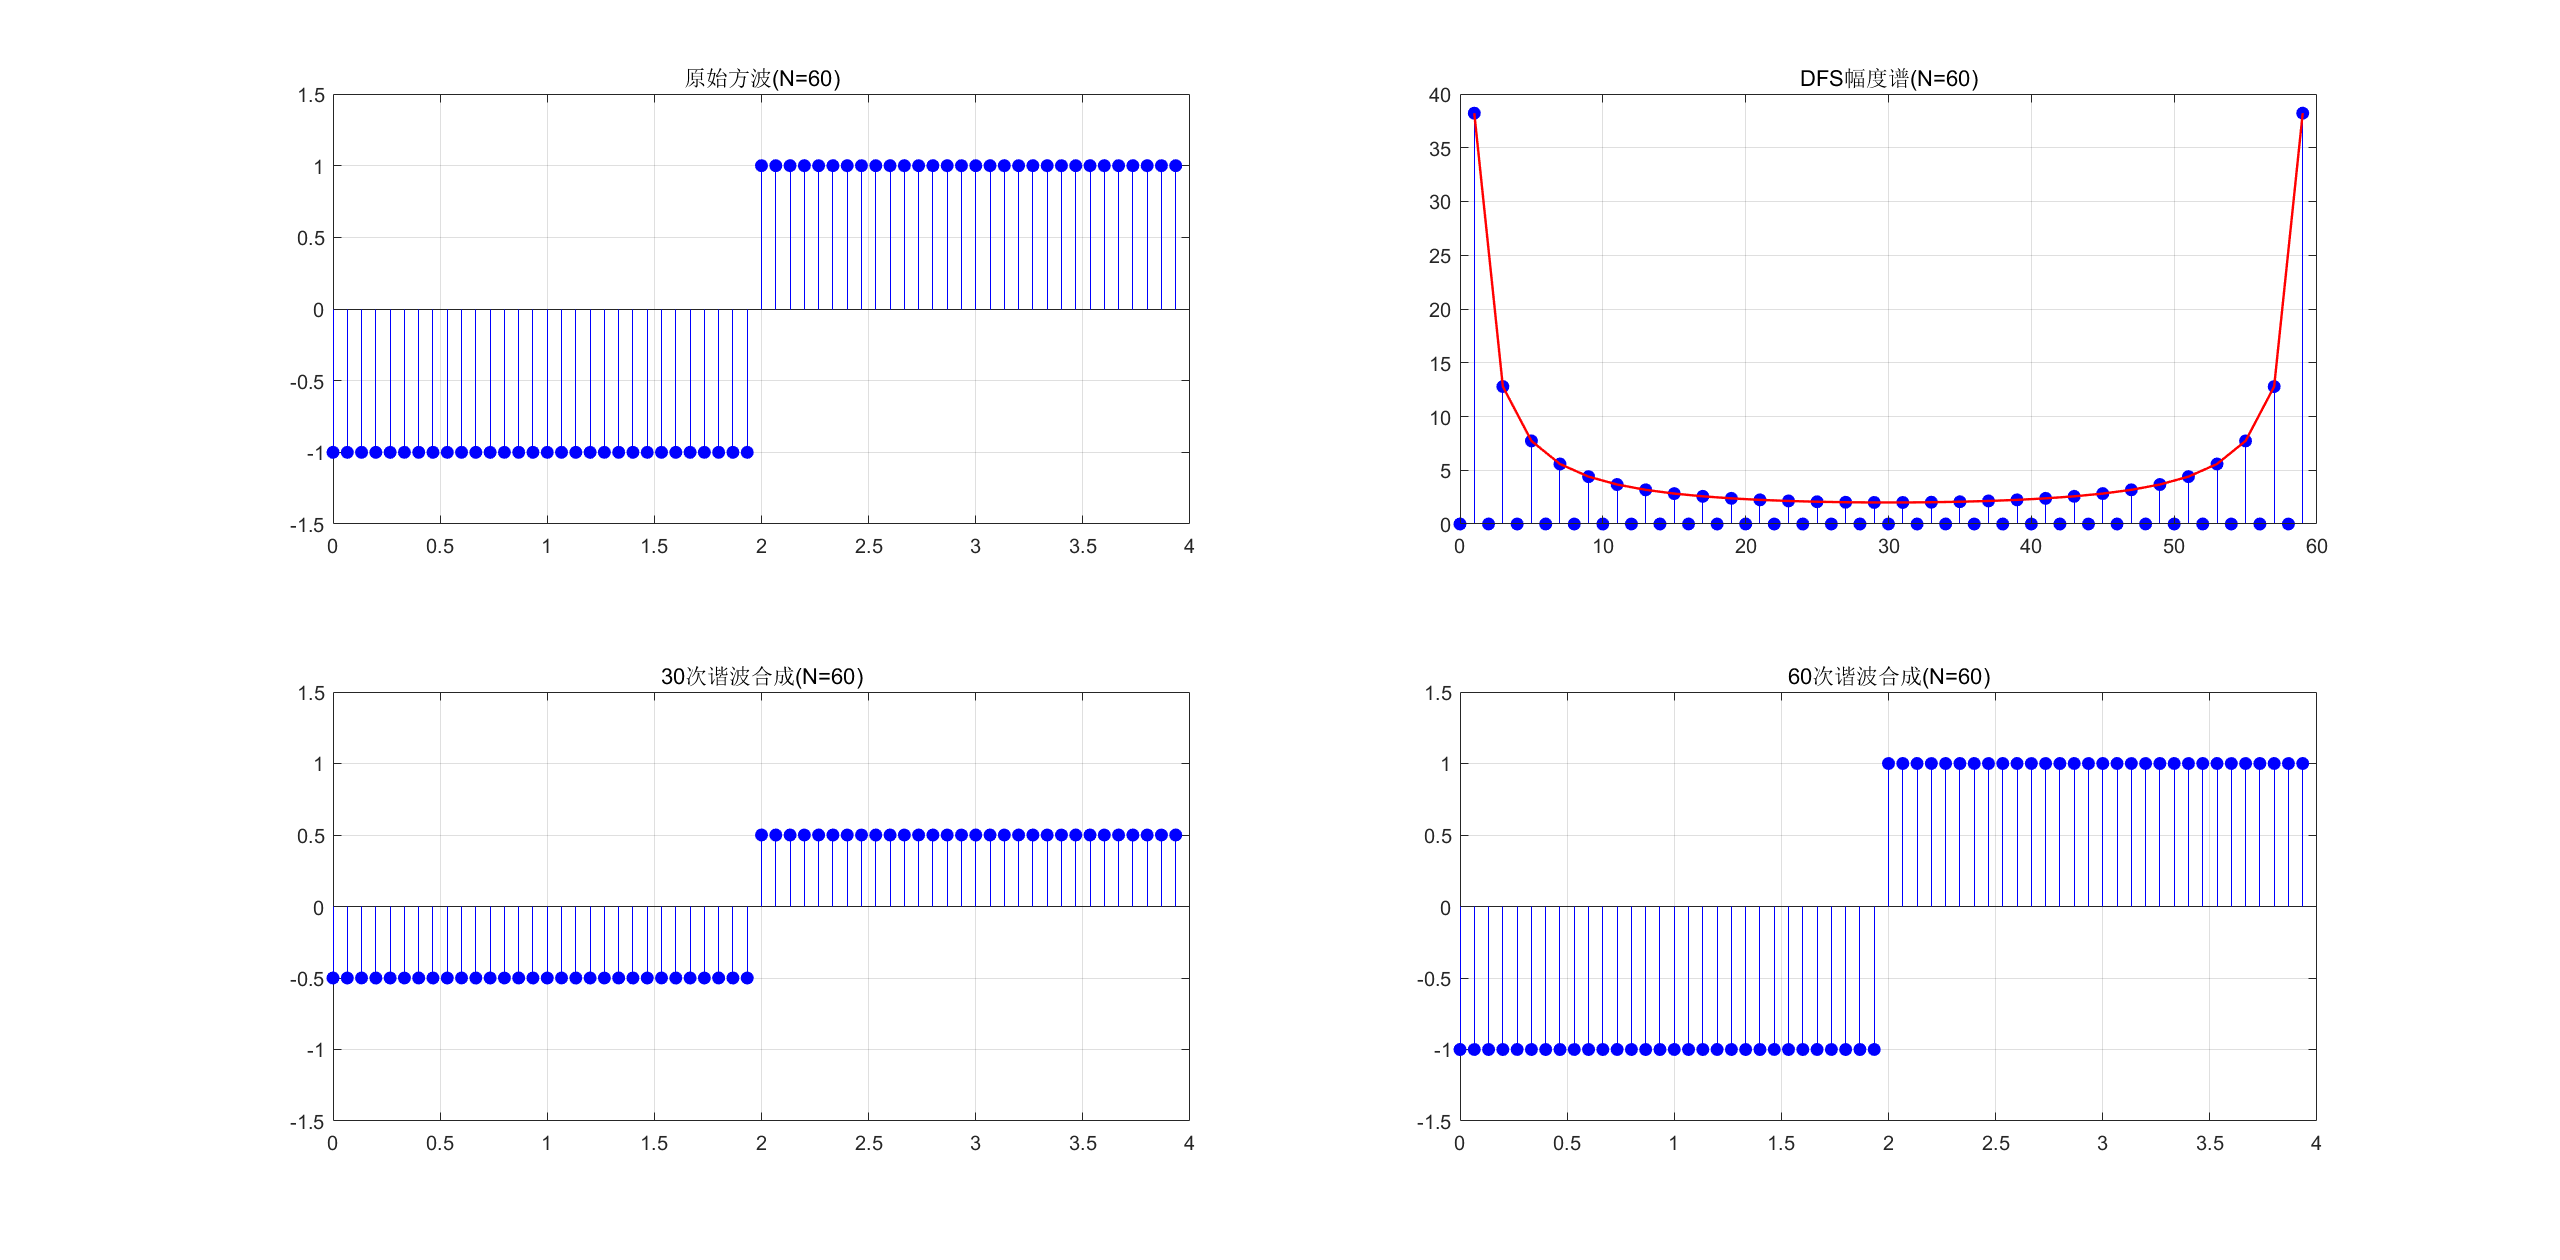
\includegraphics[width=0.8\textwidth]{1.2.1.png}
\caption{1次、1+3+5次谐波叠加波形对比}
\end{figure}

\begin{figure}[H]
\centering
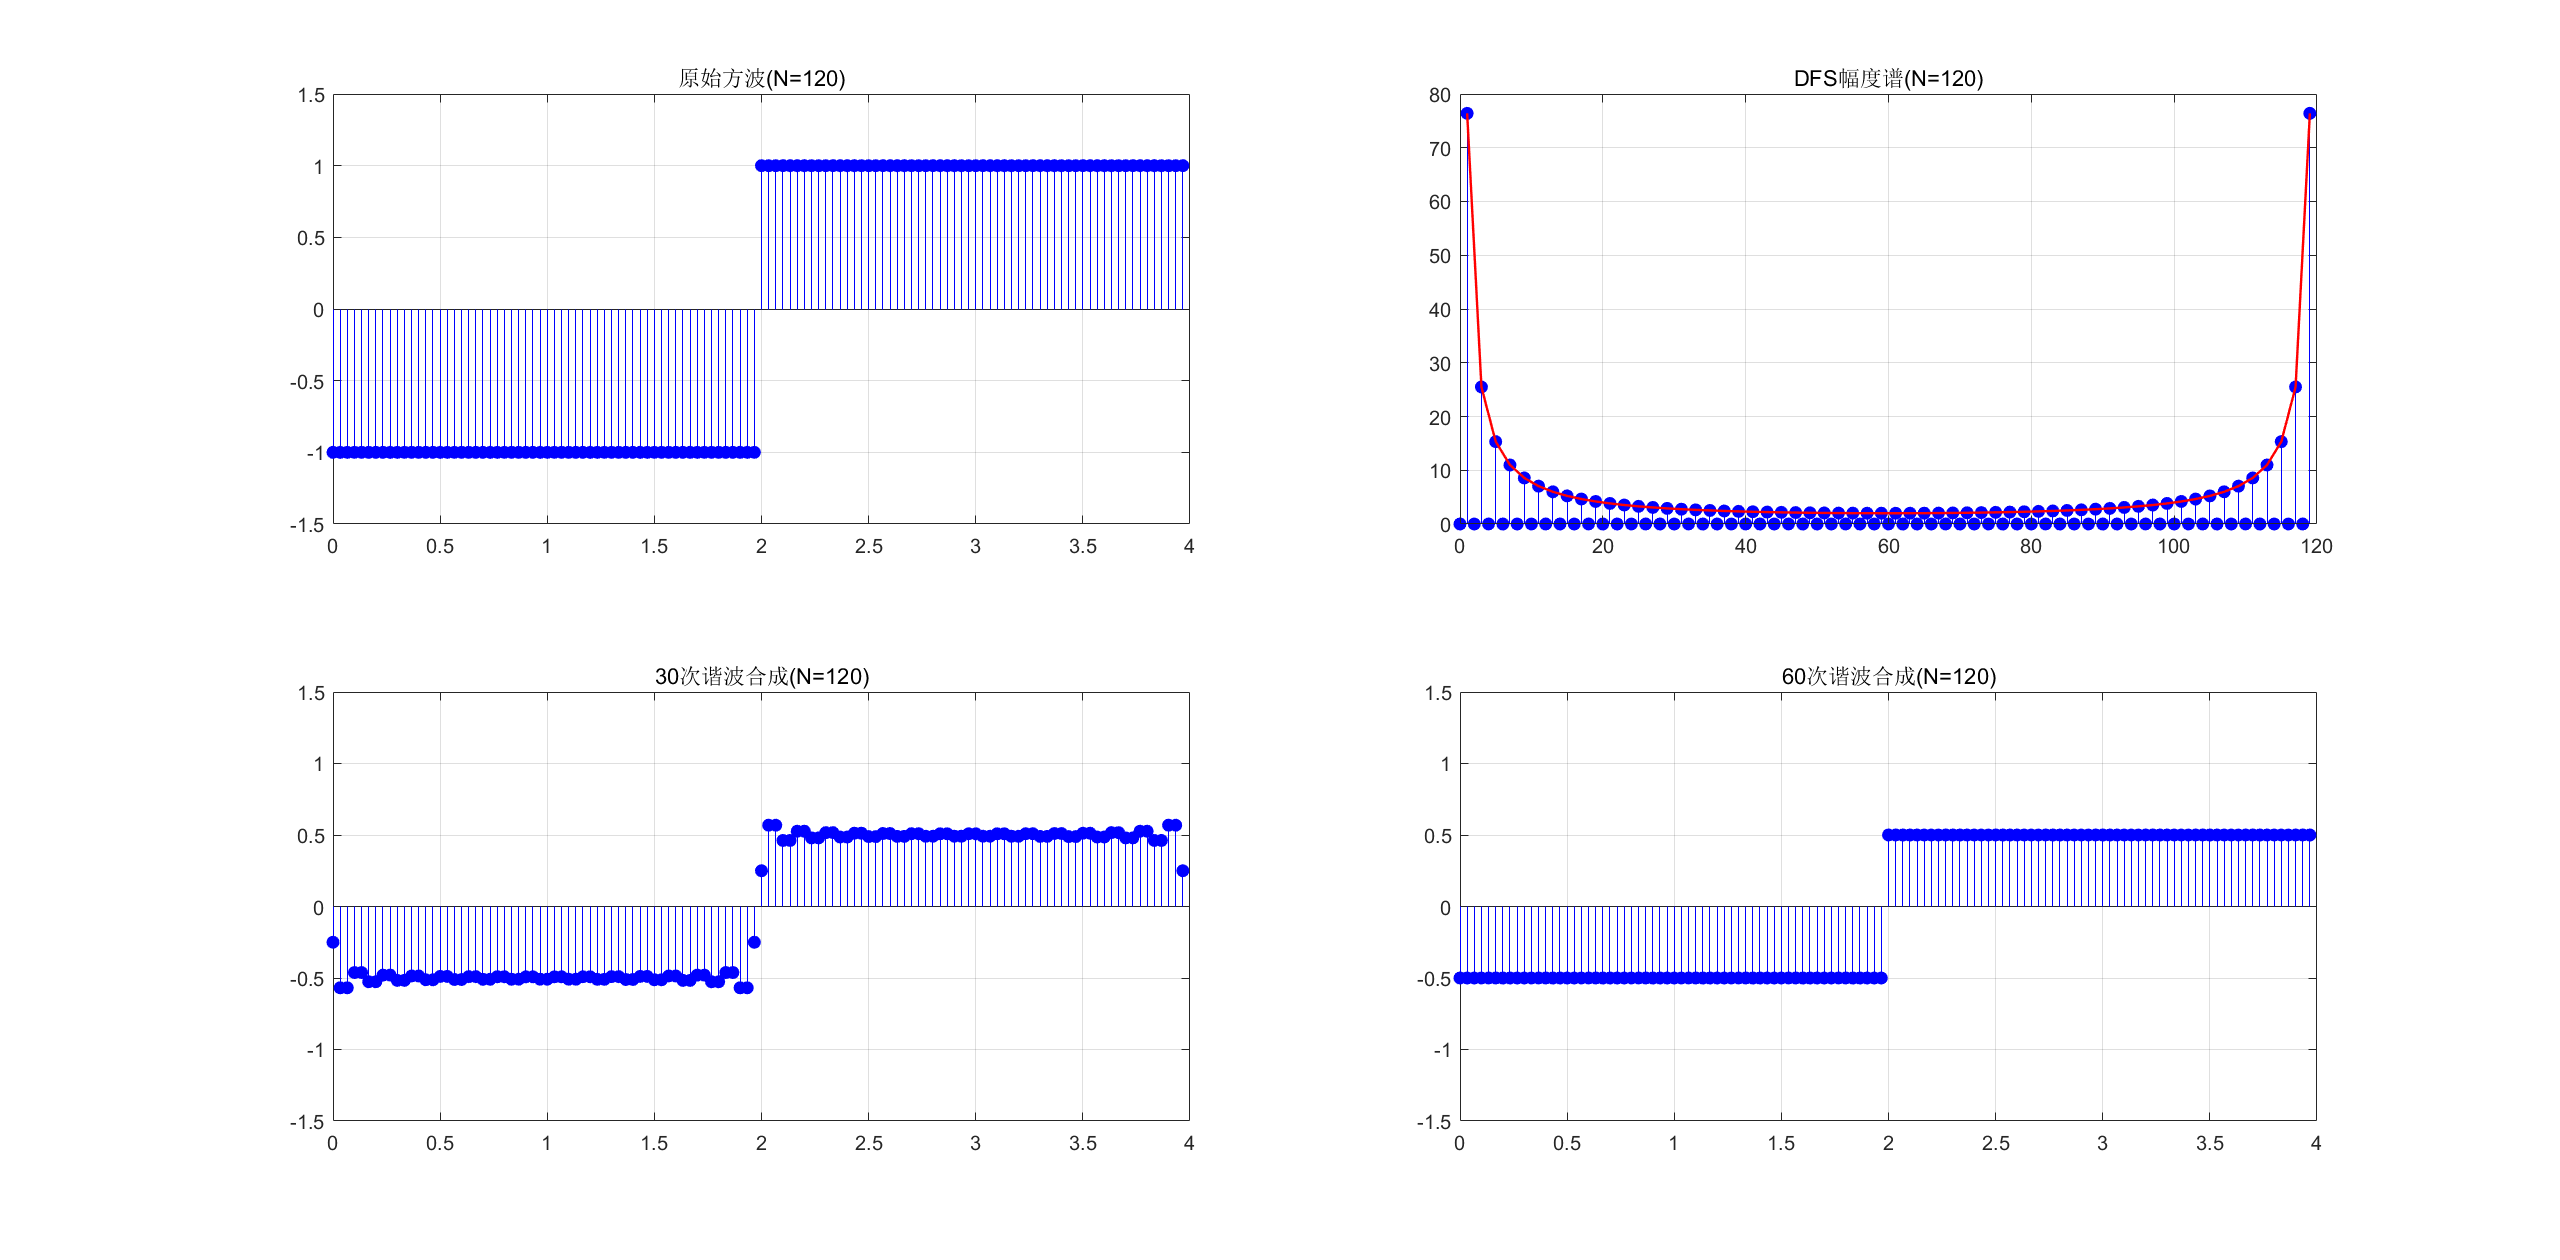
\includegraphics[width=0.8\textwidth]{1.2.2.png}
\caption{49次、501次谐波叠加（吉布斯现象）}
\end{figure}

\begin{figure}[H]
\centering
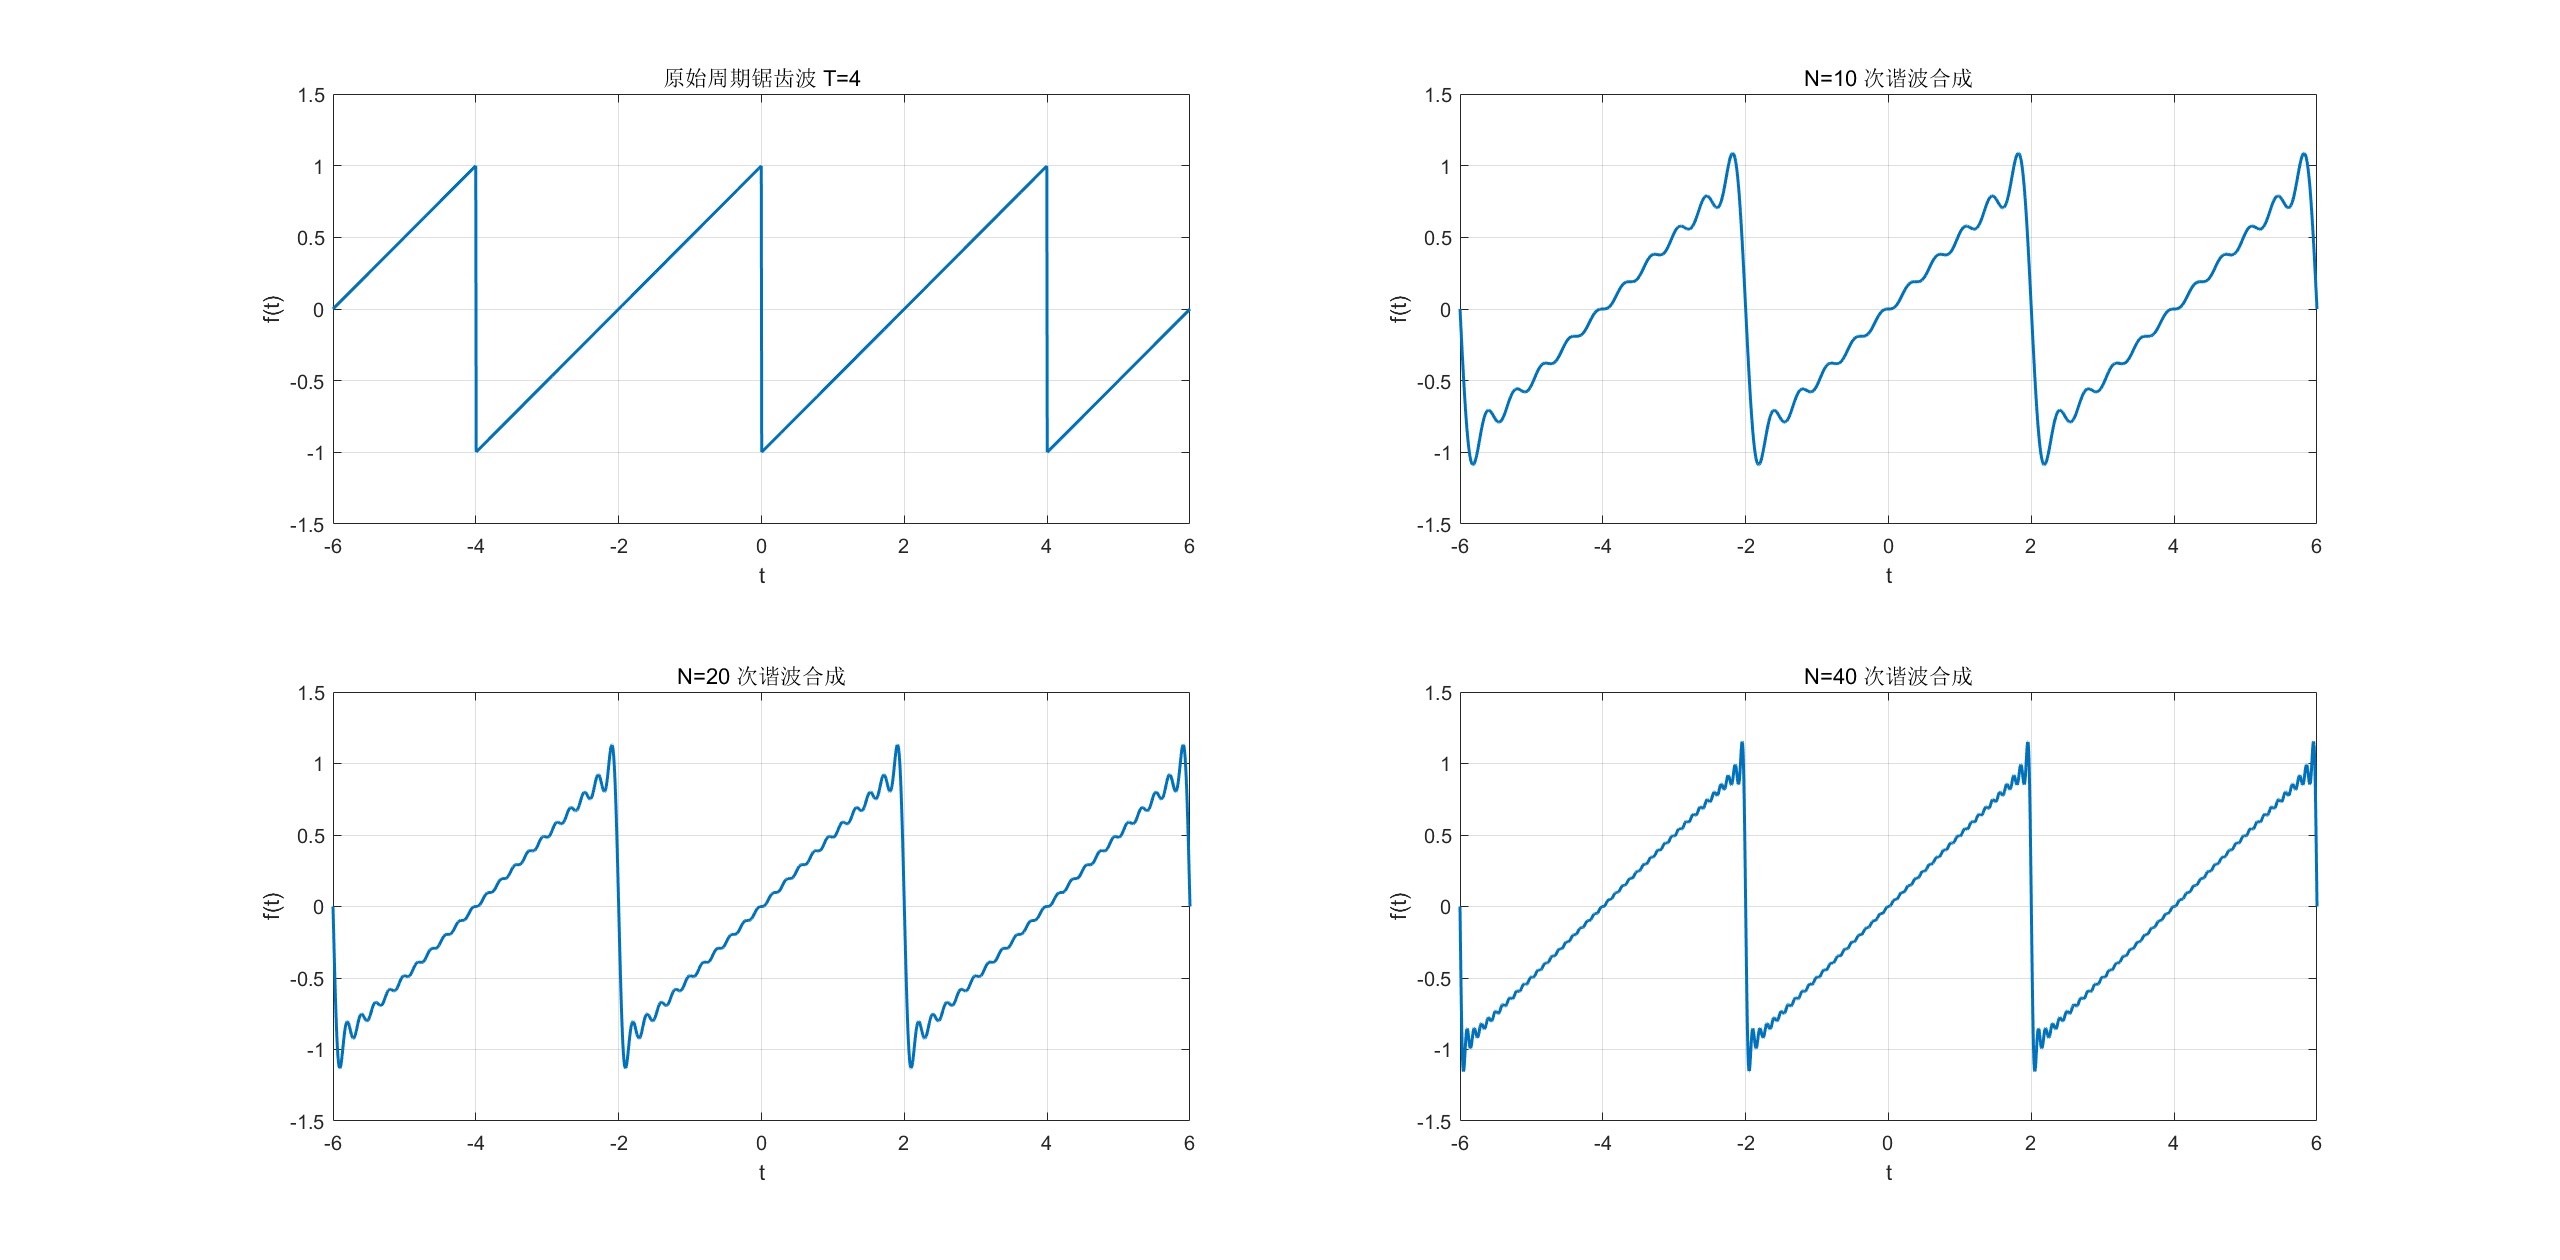
\includegraphics[width=0.8\textwidth]{1.3.png}
\caption{周期锯齿波原信号与7次谐波合成对比}
\end{figure}

\subsection{三、完整MATLAB源代码}
\subsubsection{1. 连续周期方波傅里叶级数合成程序（主程序+自定义函数）}
\begin{lstlisting}
% exp1_con_square.m
clear; clc; close all;
T = 4;
omega0 = 2*pi/T;
t = linspace(0,8,1000);

%生成原始周期方波
f_ori = zeros(size(t));
for ii = 1:length(t)
    rt = mod(t(ii),T);
    if rt < 2
        f_ori(ii) = -1;
    else
        f_ori(ii) = 1;
    end
end

%不同阶次谐波合成
f1 = fourier_square(t,omega0,1);
f3 = fourier_square(t,omega0,5);
f49 = fourier_square(t,omega0,49);
f501 = fourier_square(t,omega0,501);

%四张子图
figure('Name','连续方波谐波合成');
subplot(2,2,1);plot(t,f_ori,'k',t,f1,'r--');grid on;title('N=1次谐波');xlabel('t(s)');
subplot(2,2,2);plot(t,f_ori,'k',t,f3,'r--');grid on;title('N=1,3,5次谐波');xlabel('t(s)');
subplot(2,2,3);plot(t,f_ori,'k',t,f49,'r--');grid on;title('N=1~49次谐波');xlabel('t(s)');
subplot(2,2,4);plot(t,f_ori,'k',t,f501,'r--');grid on;title('N=1~501次谐波');xlabel('t(s)');

%自定义傅里叶级数合成函数
function f = fourier_square(t,w0,Nmax)
    f = zeros(size(t));
    for n = 1:2:Nmax
        bn = -4/(n*pi);
        f = f + bn*sin(n*w0*t);
    end
end
\end{lstlisting}

\subsubsection{2. 周期锯齿波分解与合成代码}
\begin{lstlisting}
% exp1_saw.m
clear; clc; close all;
T = 4; w0 = 2*pi/T;
t = linspace(0,8,2000);
%锯齿波 f(t)=0.5mod(t,T)-1
x_ori = 0.5*mod(t,T)-1;
N = 7;
xs = zeros(size(t));
for n = 1:N
    cn = ((-1)^(n+1))*2/(n*pi);
    xs = xs + cn*sin(n*w0*t);
end

figure;
plot(t,x_ori,'r-',t,xs,'b-','LineWidth',1);
grid on;legend('原始锯齿波','7次谐波合成');
title('周期锯齿波分解合成');xlabel('t(s)');ylabel('f(t)');
\end{lstlisting}

\subsubsection{3. 离散方波DFS/IDFS分解合成（双采样间隔+自定义DFS/IDFS）}
\begin{lstlisting}
% exp1_dis_square.m
clear; clc; close all;
T = 4;
N1 = 6*T; Ts1 = T/N1;
N2 = 12*T;Ts2 = T/N2;

%生成两种离散序列
t1 = linspace(0,T,N1,'Endpoint',false);
t2 = linspace(0,T,N2,'Endpoint',false);
x1 = double(mod(t1,T)>=2)-double(mod(t1,T)<2);
x2 = double(mod(t2,T)>=2)-double(mod(t2,T)<2);

%自定义DFS、IDFS
function X = dfs(x)
    N = length(x);
    X = zeros(1,N);
    for k = 0:N-1
        sm = 0;
        for n = 0:N-1
            sm = sm + x(n+1)*exp(-1j*2*pi*k*n/N);
        end
        X(k+1)=sm;
    end
end
function x = idfs(X)
    N = length(X);
    x = zeros(1,N);
    for n = 0:N-1
        sm = 0;
        for k = 0:N-1
            sm = sm + X(k+1)*exp(1j*2*pi*k*n/N);
        end
        x(n+1)=sm/N;
    end
end

%求频谱与谐波还原
X1 = dfs(x1);A1 = abs(X1);
X2 = dfs(x2);A2 = abs(X2);
%截取前30、60点做IDFS
x30_1 = real(idfs([X1(1:30),zeros(1,N1-30)]));
x60_2 = real(idfs([X2(1:60),zeros(1,N2-60)]));

%绘图
figure('Name','离散方波DFS分析');
subplot(2,2,1);stem(0:N1-1,x1,'filled');title('Ts=T/6原始离散序列');grid on;
subplot(2,2,2);stem(0:N1-1,A1,'filled');title('对应幅度谱');grid on;
subplot(2,2,3);stem(0:N2-1,x2,'filled');title('Ts=T/12原始离散序列');grid on;
subplot(2,2,4);stem(0:N2-1,A2,'filled');title('对应幅度谱');grid on;
\end{lstlisting}

\subsection{四、实验思考题}
\begin{enumerate}
    \item 结合理论与实验结果，简述连续周期信号频谱的特点。
    \textbf{答：(1) 离散性：频谱仅在基波整数倍频率点上存在谱线，为离散线状谱；(2) 谐波性：谱线位置为$nf_0,n=0,1,2\cdots$；(3) 收敛性：谱线幅值随谐波次数升高整体衰减，高频分量逐步减小。}
    
    \item 结合理论与实验结果，简述离散周期信号频谱的特点。
    \textbf{答：(1) 离散性：DFS频谱在一个周期内为N根离散谱线；(2) 周期性：频谱以$2\pi$为周期无限重复延拓；(3) 有限性：仅N个独立谐波分量，无无穷次谐波。}
    
    \item 周期矩形脉冲：周期$T$、脉宽$\tau$变化如何影响频谱？离散序列采样间隔变化对频谱的影响？
    \textbf{答：连续：$T$变大→谱线变密；$\tau$变小→频谱主瓣带宽增大、衰减变慢。离散：采样间隔增大→等效采样频率降低，易发生频谱混叠；采样间隔减小→采样频率提高，频谱混叠被抑制。}
\end{enumerate}